\subsection{Beamline} \label{sec:beamline}
The CLAS12 beamline geometry is entirely imported from the engineering CAD model.
It is made up of several pieces, each discussed below. The positioning and composition of the beamline
depends on the run configuration, which can be:

\begin{itemize}
	\item FTOn: Forward Tagger present and operational. The M\"oller shield starts at $z$=877 mm from the target center (see \F{beamlineGeometry} top).
	\item FTOff: FT is present but not operational. The FT tracker is replaced by an additional shielding.
                 The M\"oller shield starts at $z$=430 mm from the target center, and additional shielding
                 is present to connect it to the FT (see \F{beamlineGeometry} bottom).
\end{itemize}


\begin{figure}
	\centering
	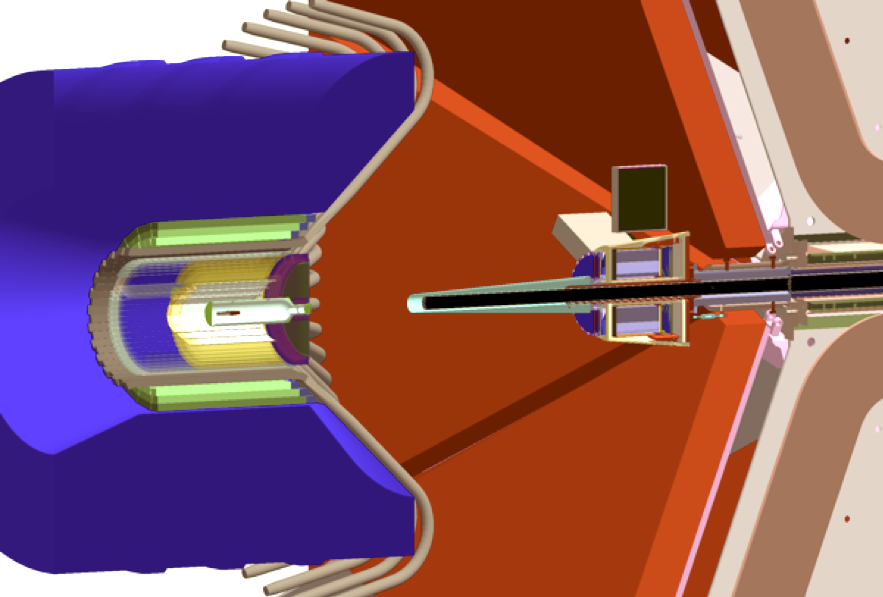
\includegraphics[width=0.99\columnwidth,keepaspectratio]{img/ftOnGeometry.png}
	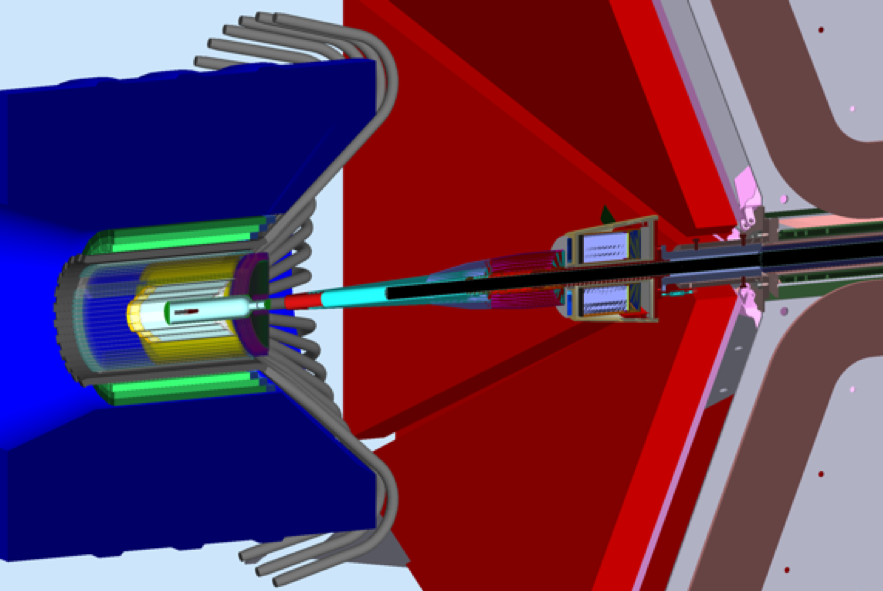
\includegraphics[width=0.99\columnwidth,keepaspectratio]{img/ftOffGeometry.png}
	\caption{The two possible CLAS12 FT beamline configurations. Top: FTOn. To clear its acceptance at forward angles (2.50\mdeg-4.50\mdeg),
             the M\"oller shield (cyan color) is attached to the FT tracker, starting at $z$=877 mm from the target.
             Bottom: FToff; the FT is present but not operational. The FT tracker is replaced with a shield.
             The M\"oller cone is placed at $z$=430 mm from the target and additional shielding
             is added to minimize background in region 1 DC.}
	\label{fig:beamlineGeometry}
\end{figure}

\subsubsection{Vacuum Pipe}

The beamline is given by a stainless steel vacuum pipe that contains the electron beam.
The pipe starts downstream of the target at $z$=80 cm and changes dimensions inside
the torus and downstream of the torus as detailed in Table \ref{tab:beampipe}.

\begin{table}[h]
	\begin{center}
		\begin{tabular}{| c | c | c |}
			\hline \hline
			                & Thickness (mm) & Inner Radius (mm)   \\
			\hline
              Upstream      &    1.6     &    26.9 \\
              Inside        &    1.6     &    33.3 \\
            Downstream      &    3.2     &    60.3 \\
			\hline \hline
		\end{tabular}
	\end{center}
	\caption{The vacuum beampipe dimensions upstream, inside, and downstream of the torus.}\label{tab:beampipe}
\end{table}


\subsubsection{M\"oller Shielding}
The M\"oller shielding is composed of the following elements, shown in \F{moellerShieldingFTOn} for the FTOn configuration
and in \F{moellerShieldingFTOff} for the FTOff configuration.

\begin{figure}
	\centering
	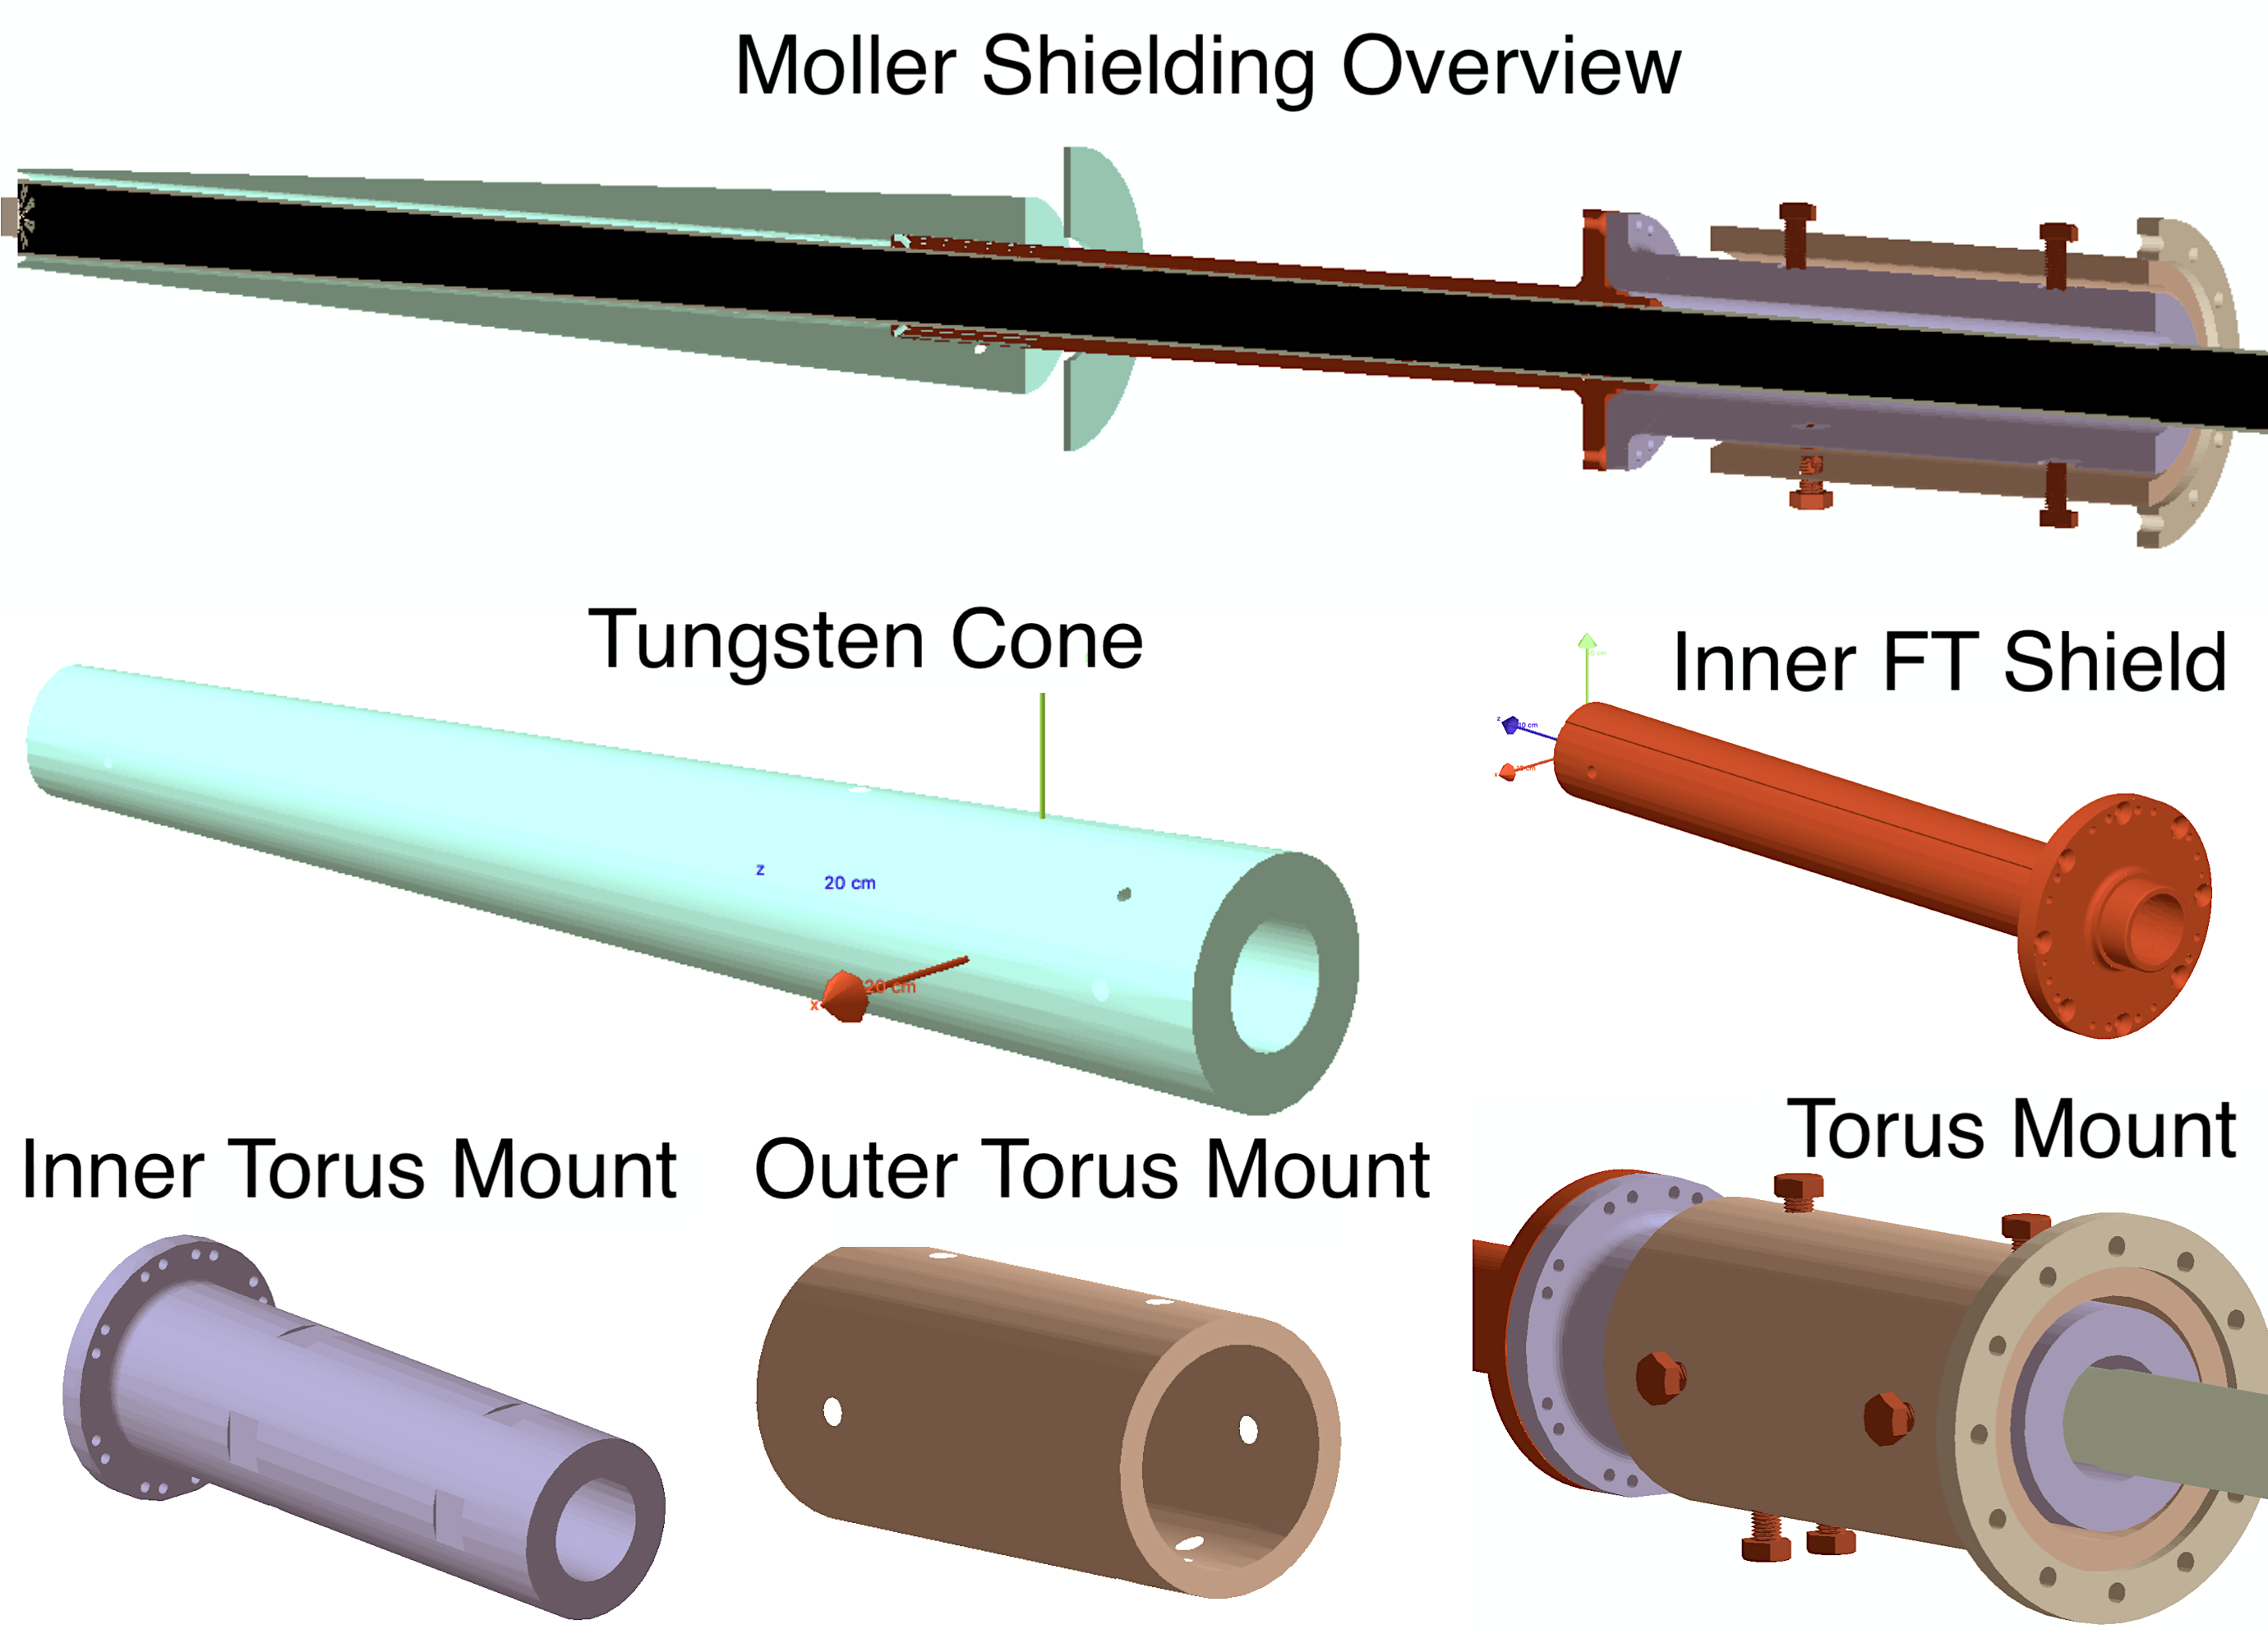
\includegraphics[width=0.99\columnwidth,keepaspectratio]{img/moellerShieldingFTOn.png}
	\caption{The M\"oller shielding for the FTOn configuration implemented in GEMC. On top a section of the overall overview of the cone, FT support, and torus mount.
		     Various individual components are shown: the tungsten cone, the inner FT shield, and the structure of the torus mount.}
	\label{fig:moellerShieldingFTOn}
\end{figure}

\begin{figure}
	\centering
	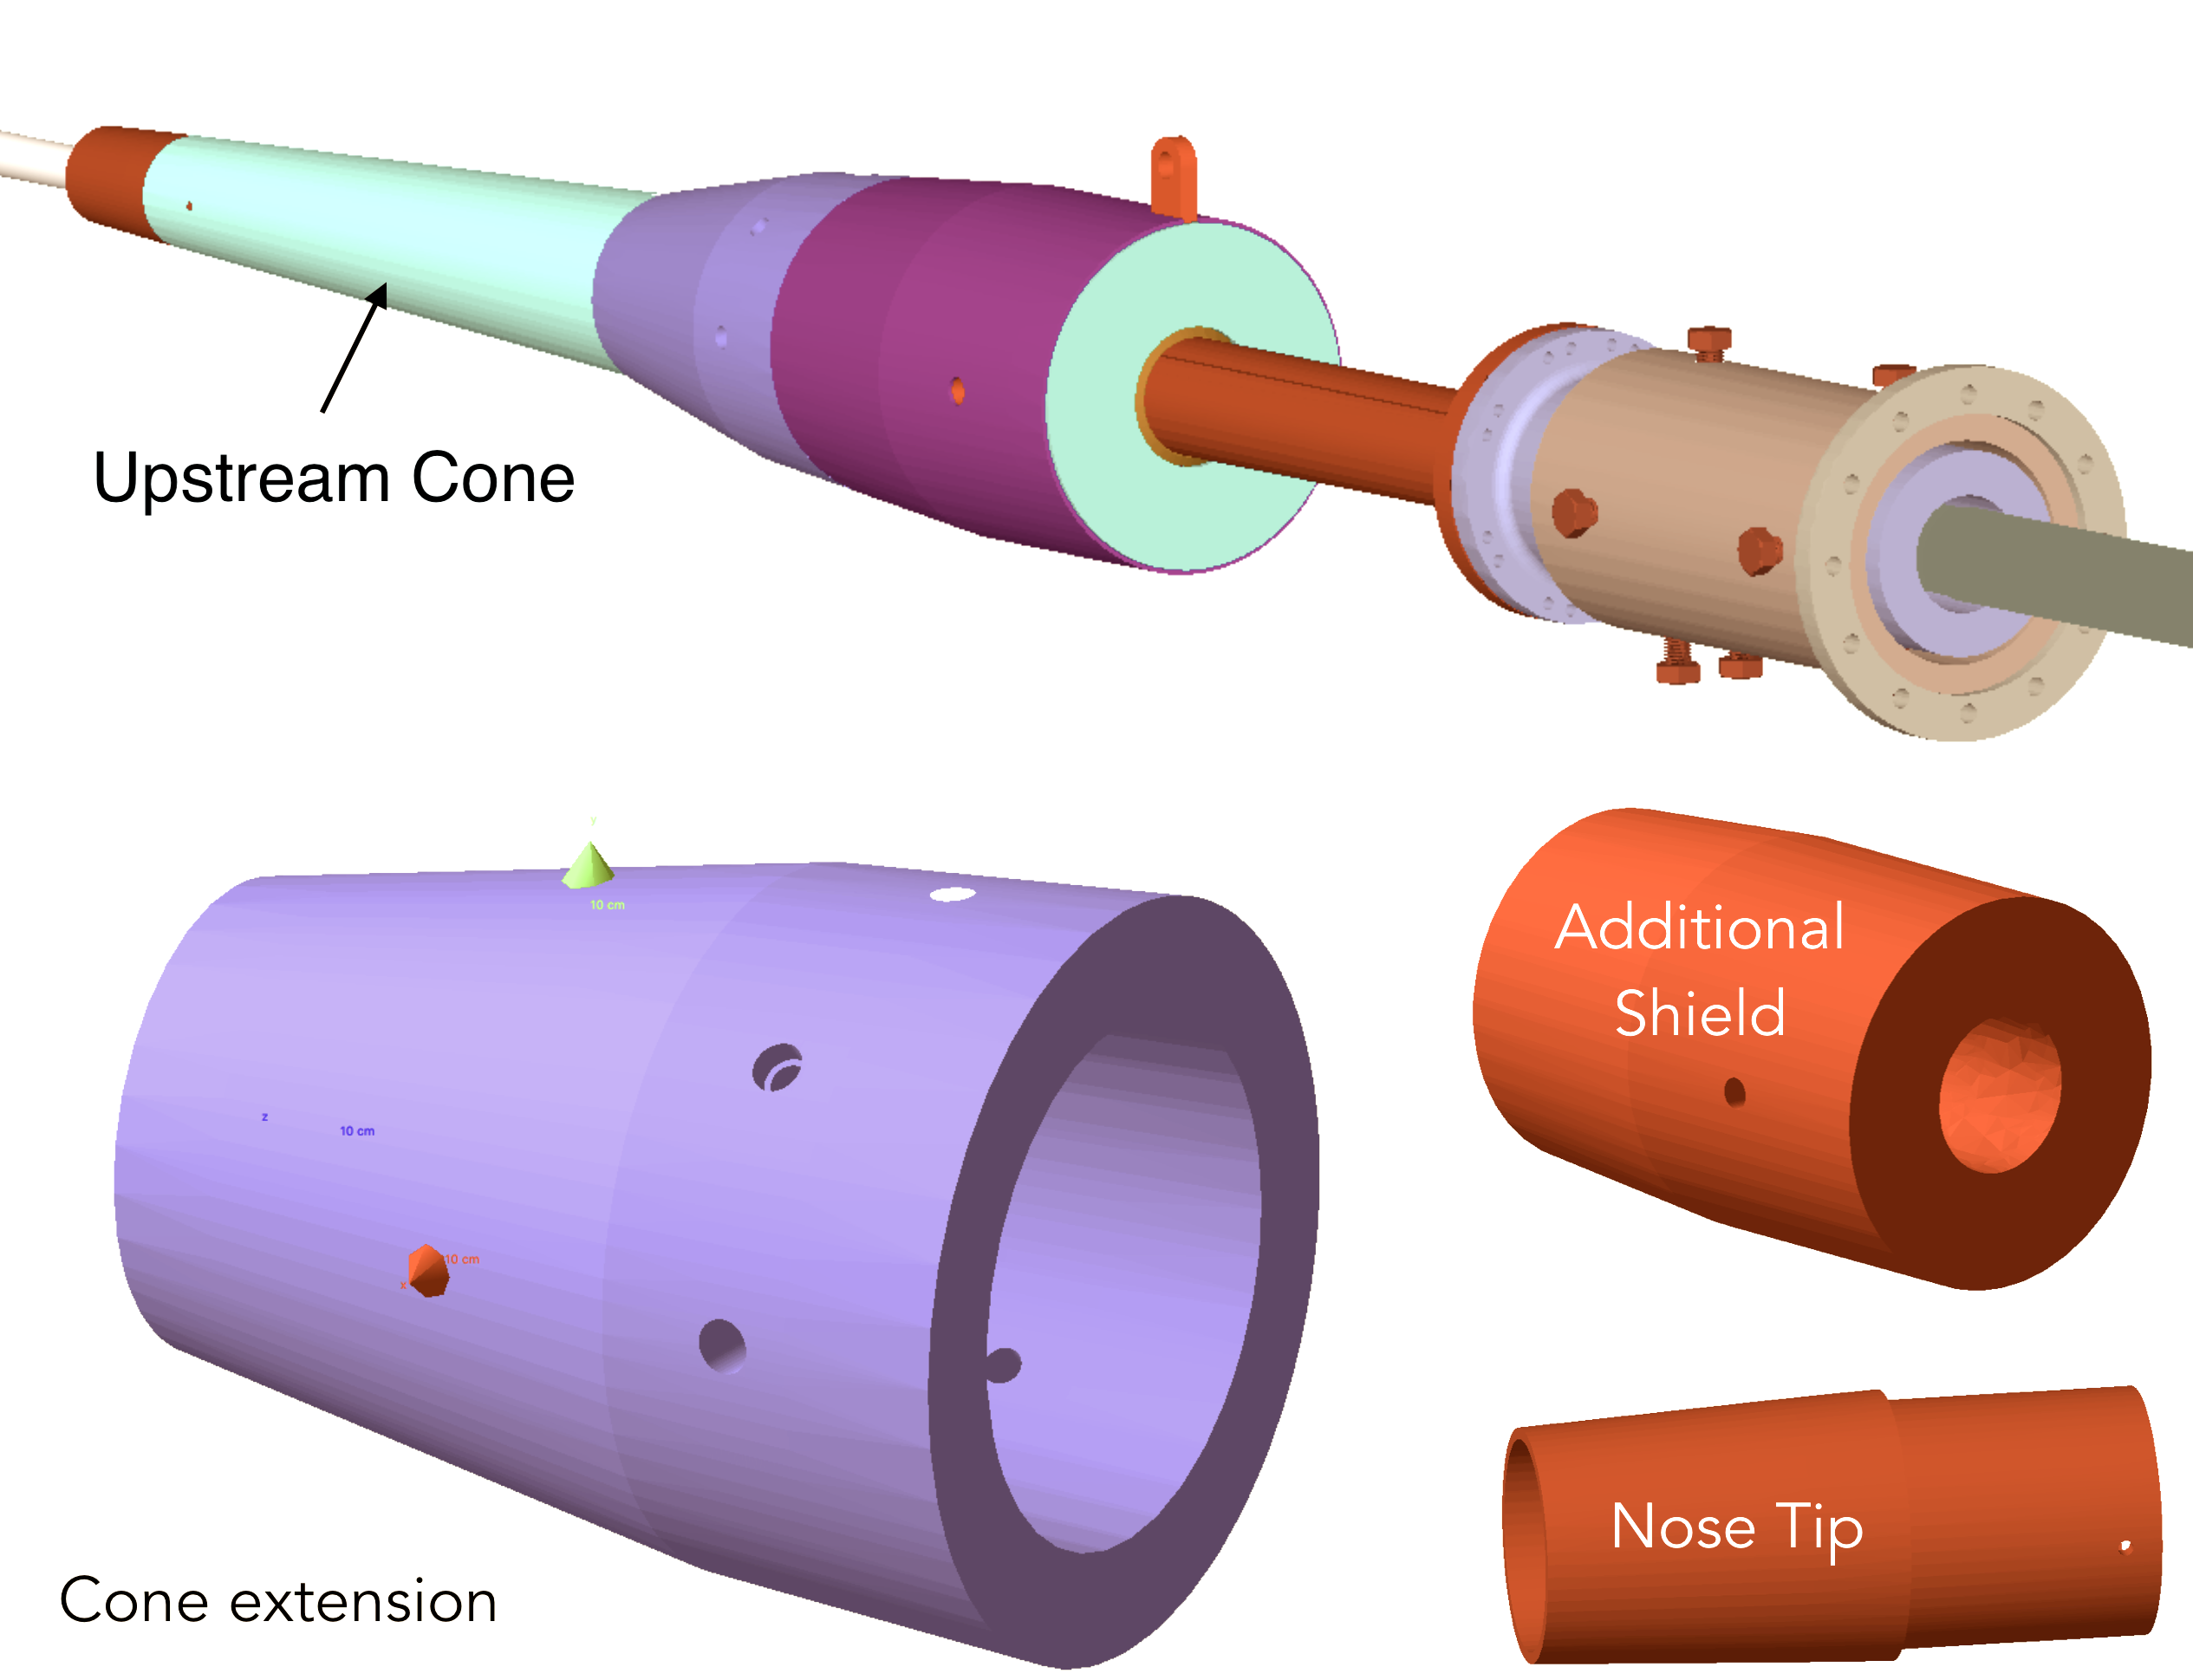
\includegraphics[width=0.99\columnwidth,keepaspectratio]{img/moellerShieldingFTOff.png}
   \caption{The M\"oller shielding for the FTOff configuration implemented in GEMC. Top: section of the overall overview of the cone, FT support, and torus mount.
            The cone tip extension and the additional shielding that replaces the FT tracker are also shown.}
	\label{fig:moellerShieldingFTOff}
\end{figure}



\begin{itemize}
	\item FTOn and FTOff configurations:
	\begin{itemize}
		\item a tungsten cone with increasing thickness
		\item a tungsten pipe and flange inside the FT
		\item a support system to mount the FT and the shielding onto the torus frame, composed by:
		\begin{itemize}
			\item an inner stainless steel shield and flange
			\item an outer tungsten shield
			\item nine copper screws to adjust the alignment of the FT and shields upstream of the torus
		\end{itemize}
	\end{itemize}
	\item Additions for FTOff configuration:
	\begin{itemize}
	\item a tungsten cone tip to extend the M\"oller shield cone
	\item lead cylinder in place of the FT tracker
	\end{itemize}

\end{itemize}




\subsubsection{Torus and Downstream Shielding}
Additional shielding is placed around the vacuum pipe through the torus magnet bore in the form of tungsten cylinders.
Shielding downstream of the torus in the form of a connecting tungsten nose and a long lead cylinder enclosed
by a stainless steel frame is also included \cite{beamline-nim}.
